\documentclass[10pt]{beamer}

\usepackage{fontspec}
\setmainfont{Ubuntu}[]
\setsansfont{Ubuntu}[]
\setmonofont{Ubuntu Mono}[]

\usepackage{graphicx}
\graphicspath{ {../img/} }

\usepackage[absolute,overlay]{textpos} % [showboxes]

\beamertemplatenavigationsymbolsempty

\title{Иммутабельность}

\begin{document}

\begin{frame}
  \frametitle{Польза иммутабельности}
  \begin{itemize}
  \item исключает ошибки с изменением одних и тех же данных из разных мест в коде;
  \item в том числе из разных потоков;
  \item упрощает сборку мусора;
  \item компилятор имеет больше возможностей для оптимизации;
  \item статический анализатор имеет больше возможностей для проверки корректности.
  \end{itemize}
\end{frame}

\begin{frame}
  \frametitle{Данные и указатель}
  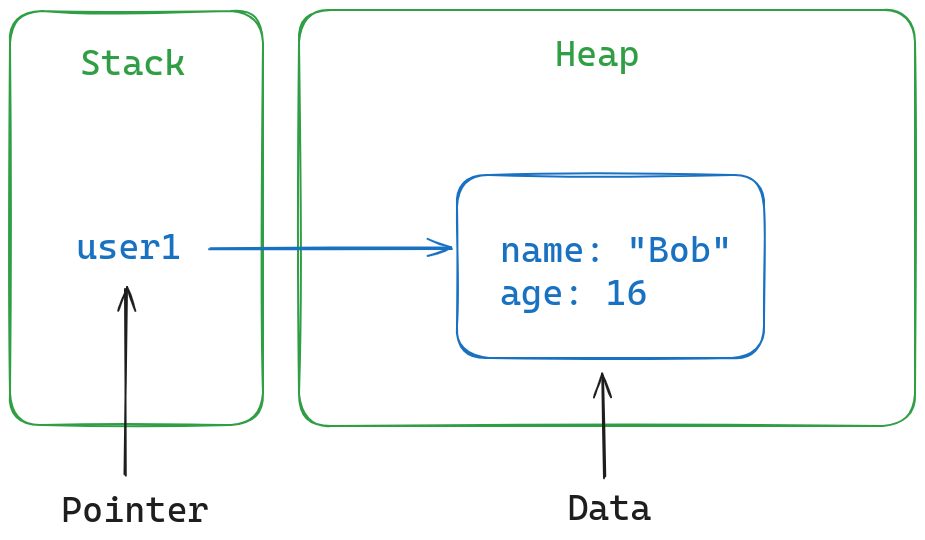
\includegraphics[scale=0.33]{data_and_pointer}
\end{frame}

\begin{frame}
  \frametitle{4 варианта иммутабельности}
  \begin{itemize}
  \item мутабельные данные, мутабельный указатель
  \item иммутабельные данные, мутабельный указатель
  \item иммутабельные данные, иммутабельный указатель
  \item мутабельная память, иммутабельный указатель
  \end{itemize}
\end{frame}

\begin{frame}
  \frametitle{4 варианта иммутабельности}
  \begin{itemize}
  \item большинство императивных языков
  \item Эликсир
  \item Эрланг
  \item не имеет смысла на практике
  \end{itemize}
\end{frame}

\begin{frame}
  \frametitle{Переиспользование памяти}
  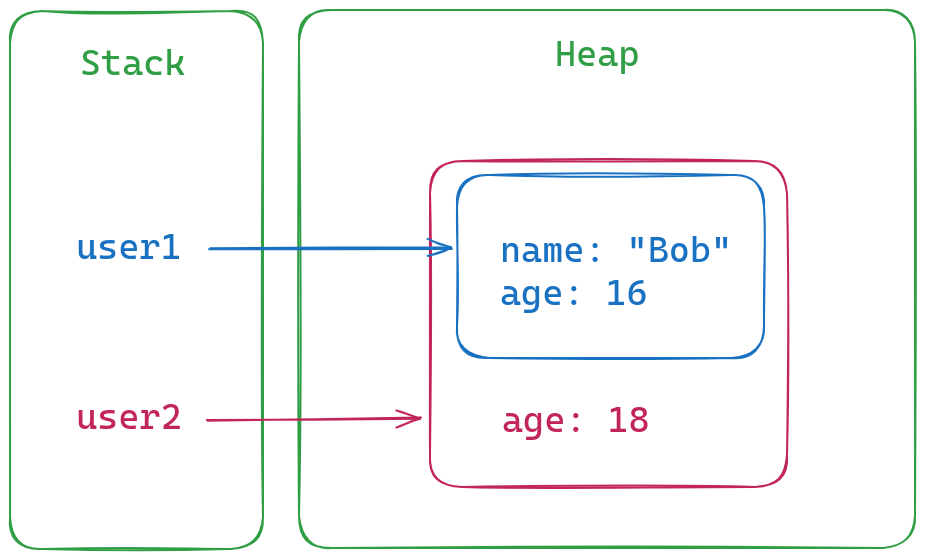
\includegraphics[scale=0.33]{structure_sharing}
\end{frame}

\end{document}
